\documentclass[11pt]{article}
\usepackage[utf8]{inputenc}
\usepackage[T1]{fontenc}
\usepackage[top=1.1cm,bottom=1.3cm,left=1.8cm,right=1.8cm]{geometry}
\usepackage{titlesec}
\usepackage{enumitem}
\usepackage{parskip}
\usepackage{graphicx}
\usepackage{float}

\titleformat{\section}{\large\bfseries}{\thesection}{0.6em}{}
\titleformat{\subsection}{\normalsize\bfseries}{\thesubsection}{0.6em}{}
\setlist{itemsep=1pt, topsep=2pt, partopsep=0pt, parsep=0pt}
\setlength{\parskip}{3pt}

\usepackage{fancyhdr}
\pagestyle{fancy}
\fancyhf{}
\fancyhead[R]{June 12, 2026}
\renewcommand{\headrulewidth}{0pt}

\begin{document}
\vspace{-1.8cm}
\begin{center}
{\LARGE\textbf{Phone-to-3D Project: Technical Report}}\\[0.3cm]
Nil Sıla Ulucan, Tibet Gül
\end{center}
\vspace{-0.4cm}

\section{Introduction and Project Goal}
Phone-to-3D is an open-ended computer vision pipeline that automatically
reconstructs a 3D point cloud and mesh model from a sequence of photos
captured with a phone camera. The core goal of the project is to obtain a 3D
digital twin of a real-world scene or object using only ordinary
phone-camera imagery, without any additional hardware such as LiDAR or
depth sensors, by applying Structure-from-Motion (SfM) and Multi-View
Stereo (MVS) techniques. The pipeline is implemented as a command-line
Python application. Its primary and currently validated workflow is
photo-to-3D: it takes a folder of still images (e.g. the Gerard Hall
benchmark dataset) and reconstructs a 3D model directly from them. As an
additional input mode, the codebase also supports extracting frames from a
video file via FFmpeg and feeding those frames into the same pipeline, but
this path has not yet been validated end-to-end.

\section{System Architecture and Pipeline Stages}
The project is built around a four-stage end-to-end flow defined in
\texttt{src/pipeline/full\_pipeline.py}:

\subsection{1. Input Handling (Direct Image Set or Video to Frames)}
In the primary, validated workflow the input is already a directory of
photos (e.g. a static benchmark dataset such as Gerard Hall), so this step is
skipped entirely and the images are passed directly to the SfM stage. As an
optional secondary path, the \texttt{video\_to\_frames.py} module can use
FFmpeg to extract JPEG frames from an input video at a rate of 10 frames per
second (\texttt{FRAME\_RATE}) and feed those frames into the same downstream
pipeline.

\begin{figure}[H]
\centering
\vspace{-4pt}
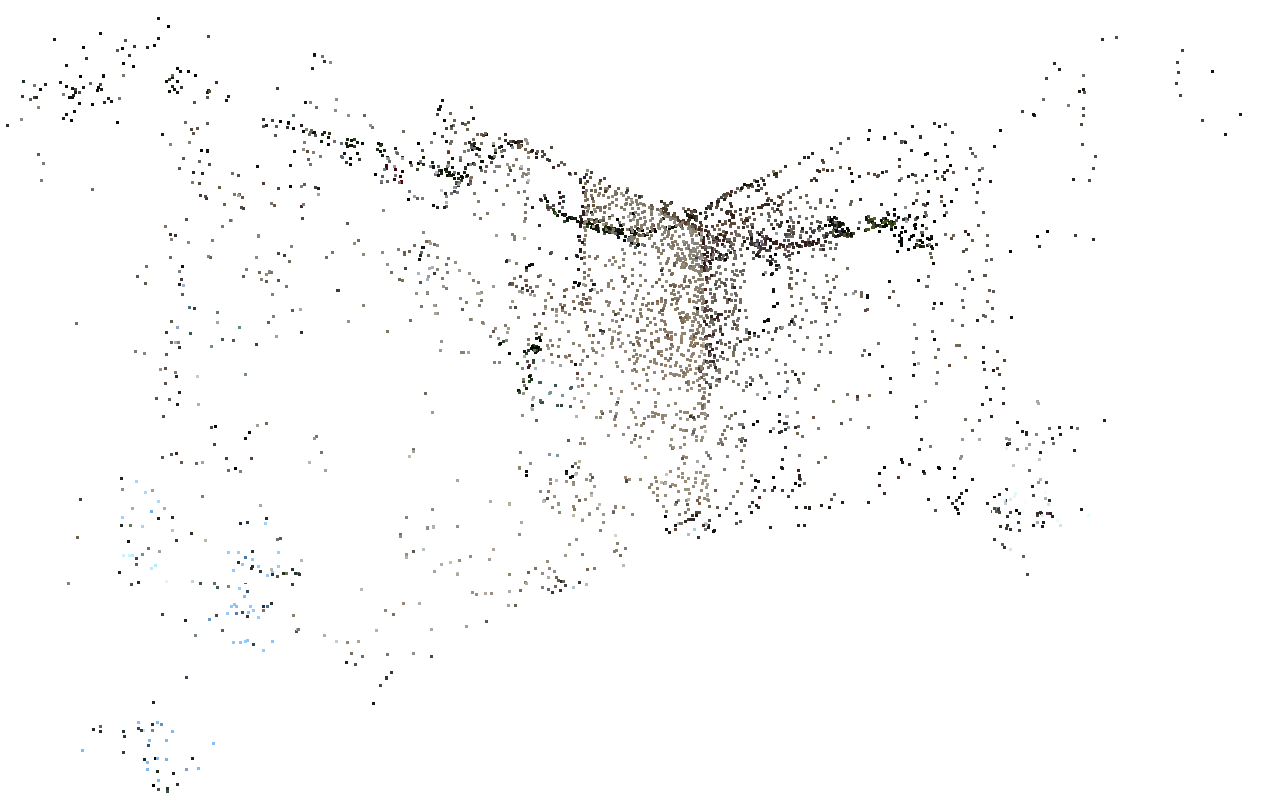
\includegraphics[width=0.38\textwidth]{sparse_pointcloud_sample.png}
\vspace{-8pt}
\caption{\small Sparse point cloud from the COLMAP SfM stage on a subset of
the Gerard Hall photo set, visualized with Open3D.}
\vspace{-8pt}
\end{figure}

\subsection{2. Sparse Reconstruction with COLMAP (SfM)}
COLMAP is run through three steps: \textit{feature\_extractor} (SIFT feature
extraction with a limit of 8192 features), \textit{exhaustive\_matcher}
(feature matching across all image pairs), and \textit{mapper} (incremental
camera pose estimation and sparse 3D point cloud generation), followed by
\textit{model\_converter} to export a human-readable TXT model. The mapper's
inlier and match-count thresholds were lowered so reconstruction does not
fail on small or weakly matched image sets.

\subsection{3. Dense Reconstruction and Mesh Generation with OpenMVS}
The OpenMVS tools (\textit{InterfaceCOLMAP}, \textit{DensifyPointCloud},
\textit{ReconstructMesh}, \textit{RefineMesh}, \textit{TextureMesh}) have been
tested manually on Windows -- the \texttt{DensifyPointCloud-*.log} files in
the repository confirm this. However, \texttt{run\_openmvs.py} does not yet
call these tools automatically: it currently only runs an emergency bypass
that converts COLMAP's sparse \texttt{points3D.bin} to \texttt{.ply} via
\textit{model\_converter}, giving a viewable sparse cloud but no dense mesh.
Automating this chain is the project's main next step.

\subsection{4. Visualization}
\texttt{src/viewer/viewer.py} loads the resulting \texttt{.ply} file with the
Open3D library and displays it in an interactive 3D window. This step is
optionally triggered from \texttt{main.py} via the \texttt{--view} flag.

\section{Project Structure: Key Files}
\begin{itemize}[itemsep=1pt, topsep=2pt]
  \item \texttt{main.py}: \texttt{argparse}-based CLI entry point with
        \texttt{--name}, \texttt{--video} and \texttt{--view} options. Also
        contains a fixed development block that runs the pipeline directly
        on the Gerard Hall photo dataset for automated testing.
  \item \texttt{src/config.py}: centralizes platform-specific
        (Windows/Unix) paths to the FFmpeg, COLMAP and OpenMVS binaries and
        the global \texttt{FRAME\_RATE} setting, so the same codebase runs on
        a Windows COLMAP install or on macOS/Linux with system-wide tools.
  \item \texttt{src/pipeline/full\_pipeline.py}: orchestrates the four
        stages (input handling, COLMAP, OpenMVS, output) and returns the path
        to the final mesh \texttt{.ply}.
  \item \texttt{src/pipeline/video\_to\_frames.py}: optional, secondary
        path that calls FFmpeg to extract frames from a video file.
  \item \texttt{src/pipeline/run\_colmap.py}: runs COLMAP's
        \textit{feature\_extractor}, \textit{exhaustive\_matcher} and
        \textit{mapper} with tuned thresholds, then exports the sparse model
        to TXT.
  \item \texttt{src/pipeline/run\_openmvs.py}: currently only runs the
        "emergency bypass" (\texttt{points3D.bin} $\to$ \texttt{.ply} via
        COLMAP); the OpenMVS dense/mesh calls are not yet wired in.
  \item \texttt{src/utils/colmap\_validator.py}: sanitizes COLMAP's
        \texttt{images.txt} (filenames only, verified existence, Unix line
        endings); written for OpenMVS's \textit{InterfaceCOLMAP} step but not
        yet called from the pipeline.
  \item \texttt{src/utils/file\_utils.py} / \texttt{logging\_utils.py}:
        small helpers for directory creation and consistent logging across
        all pipeline modules.
  \item \texttt{src/viewer/viewer.py}: loads and displays the final
        \texttt{.ply} point cloud/mesh with Open3D.
  \item \texttt{data/}: working directory tree containing \texttt{input\_images/}
        (photo datasets, e.g. Gerard Hall), \texttt{input\_video/}
        (\texttt{blake\_hall.mp4}, \texttt{gerard\_hall.mp4}),
        \texttt{frames/} (extracted frames), and \texttt{colmap/} (per-run
        COLMAP/OpenMVS workspaces and outputs).
\end{itemize}

\section{Technologies Used}
\textbf{Python 3} (orchestration/CLI), \textbf{FFmpeg} (video frame
extraction), \textbf{COLMAP} (feature extraction, matching and
Structure-from-Motion), \textbf{OpenMVS} (dense point cloud and mesh
generation), \textbf{Open3D} (point cloud visualization), and
\textbf{NumPy}/\textbf{OpenCV} (supporting image-processing dependencies).

\section{Challenges Encountered}
A major challenge was that COLMAP's model files could not be processed
directly by OpenMVS: on Windows, the path format and line-ending characters
in \texttt{images.txt} caused \textit{InterfaceCOLMAP} to crash. A fix
(\texttt{colmap\_validator.py}) was written but is not yet integrated into
the pipeline. Additionally, COLMAP's mapper failed on small or weakly matched
image sets under default thresholds; this was fixed by lowering the relevant
inlier and match-count thresholds.

\section{Next Steps}
The priority goals for the continuation of the project are:
\begin{itemize}[itemsep=1pt, topsep=2pt]
  \item \textbf{Automate the OpenMVS chain}: extend \texttt{run\_openmvs.py}
        to call \texttt{colmap\_validator.py}, then run
        \textit{InterfaceCOLMAP} $\rightarrow$ \textit{DensifyPointCloud}
        $\rightarrow$ \textit{ReconstructMesh} $\rightarrow$
        \textit{RefineMesh} $\rightarrow$ \textit{TextureMesh} via subprocess,
        as \texttt{run\_colmap.py} does for COLMAP, removing the bypass.
  \item Validate the full pipeline on real phone-recorded video samples
        (\texttt{blake\_hall.mp4}, \texttt{gerard\_hall.mp4}), and add
        automated quality metrics (point density, coverage ratio).
\end{itemize}

\end{document}
